
\documentclass[12pt,a4paper,hidelinks,fleqn]{article}            % Article 12pt font for a4 paper while hiding links
\usepackage[margin=1in]{geometry}                          % Required to adjust margins
../styleAndCommands.tex
\title{\vspace{-5ex}Assignment 1, FE5116 (2014/2015, Semester 2)\vspace{-7ex}}
\date{}
\begin{document}
\maketitle
\subsection*{Assignment 1a. Eight queens puzzle}
Write a program to place 8 chess queens on an 8x8 chessboard 
such that none of the queens is able to threaten each other.
That is, none of the queens share the same row, column or diagonal.
The solution is not unique, but your program is required to find only one valid solution.

The detailed description of the problem and possible algorithm to solve the problem can be found on wikipedia \url{http://en.wikipedia.org/wiki/Eight_queens_puzzle}.

Below is a recursive algorithm to tackle the problem.
It places the queens column by column incrementally. 
At placing column $i$, it picks a safe row against the previous placed columns ($1$ to $i-1$), 
and proceed to place the remaining columns using recursion. 
The way to check if a row $r$ is safe against the previously placed queen at ($r_p$, $c_p$) is to check if they are in the same row ($r = r_p$), the same column (by definition because we check only the previous columns), or the same diagonal ($r - i = r_p - r_p$ or $r + i = r_p + r_p$).
A solution is found if safe rows can be found all the way till the last column.
Otherwise, the algorithm rolls back and picks the next safe row at column i.
Below is the pseudo code of this algorithm.

\begin{algorithm}
	\caption{succeed = PlaceQ (prevQ, $i$)}
    \SetKwInOut{Input}{Input}
    \SetKwInOut{Output}{Output}
    \Input{prevQ: one dimensional array of length $i-1$, indicating the queens before column i are placed at (prevQ(k), k) for k $\in [1, i-1]$}
    \Output{succeed: whether it is possible to place the queens}
	\If{ $ i > 8 $} {
		solution found, print it out \\
		succeed = true;
	}
    \Else{ 
    	succeed = false; \\
    	\For{$r \gets 1$ \textbf{to} $8$} {
		  \If{ placing a queen at $(r, i)$ does not threaten prevQ} {
			\If {PlaceQ(prevQ + $(r, i)$, $i+1$) == true} {
		        succeed = true; \\
		        break; \# we are interested only in 1 solution so stop if we find one.
		        }		  
		  }
		}   
    }
\end{algorithm}

You can follow this algorithm or design your own algorithm.
But you should not brute force the problem.
The output of your program should be in this format:
\begin{verbatim}
   1   0   0   0   0   0   0   0
   0   0   0   0   1   0   0   0
   0   0   0   0   0   0   0   1
   0   0   0   0   0   1   0   0
   0   0   1   0   0   0   0   0
   0   0   0   0   0   0   1   0
   0   1   0   0   0   0   0   0
   0   0   0   1   0   0   0   0
\end{verbatim}
where $1$ represents the positions of the queens.

\paragraph{Solution}
\begin{verbatim}
function eightqueens(n)                                                                                                                      
  if (PlaceQ(n, [], 1))                                                                                                                      
    "solution found"                                                                                                                         
  else                                                                                                                                       
    "no solution found"                                                                                                                      
  end                                                                                                                                        
endfunction                                                                                                                                  
                                                                                                                                             
# check if it is safe to place a queen at (row, col)                                                                                         
# given the previous queens before column (col - 1) are placed in prevQ                                                                      
function safe = isSafe (row, col, prevQ)                                                                                                     
  safe = true;                                                                                                                               
  for i = 1:(col-1)                                                                                                                          
    # horizontal or diagonal                                                                                                                 
    if (prevQ(i) == row || prevQ(i) - i == row - col || prevQ(i) + i == row + col)                                                           
      safe = false;                                                                                                                          
    endif                                                                                                                                    
  endfor                                                                                                                                     
endfunction                                                                                                                                  
                                                                                                                                             
# place the queen for the column "col" given the previous placement
# (before col) in prevQ                                                    
function succeed = PlaceQ(n, prevQ, col)                                                                                                     
  succeed = false;                                                                                                                           
  if (col > n)                                                                                                                               
    succeed = true;                                                                                                                          
    # display solution                                                                                                                       
    solutionMat = zeros(n, n);                                                                                                               
    for i = 1:n                                                                                                                              
      solutionMat(i, prevQ(i)) = 1;                                                                                                          
    endfor                                                                                                                                   
    solutionMat                                                                                                                              
  else                                                                                                                                       
    for r = 1:n  # check each (r, col)                                                                                                       
      if ( isSafe (r, col, prevQ) ) # go to next column                                                                                      
        prevQ(col) = r;                                                                                                                      
        if ( PlaceQ(n, prevQ, col+1) )  
          succeed = true;
          return; # so that we stop when one solution is found                                                                               
        endif                                                                                                                                
      endif                                                                                                                                  
    endfor                                                                                                                                   
  end                                                                                                                                        
endfunction           
\end{verbatim}

\begin{itemize}
\item why to use a single array for \verb=prevQ=?
\item All solutions?
\end{itemize}

\subsection*{Assignment 1b. Approximation of $\pi$}
There are many infinite series for approximating $\pi$.
Implement three functions 
\begin{itemize}
\item myPi1($nTerm$): $\displaystyle \pi = 4 \sum_{k=0}^{nTerm} (-1)^{k}\frac{1}{2k+1}$
\item myPi2($nTerm$): $\displaystyle \pi = 3 + 4 \times \sum_{k=1}^{nTerm}(-1)^{k-1}\frac{1}{2k \times (2k+1) \times (2k+2)}$
\item myPi3($nTerm$): 
\begin{align*}
\pi = 4(4\arctan \frac{1}{5} - \arctan \frac{1}{239}), ~~~\text{where} 
~~~\arctan x = \sum_{k=0}^{nTerm} \frac{(-1)^k} {2k+1} x^{2k+1}
\end{align*}
\end{itemize}
and plot their convergence chart with X-axis the number of terms used $nTerm$, and Y-axis the error.

\paragraph{Solution}
\begin{verbatim}
function myPi (n)
  pi1 = myPi1(n);
  pi2 = myPi2(n);
  pi3 = myPi3(n);
  semilogy([1:length(pi1)], abs(pi1 - pi), "-r;myPi1;", 
           [1:length(pi2)], abs(pi2 - pi), "-g;myPi2;",
           [1:length(pi3)], abs(pi3 - pi), "-b;myPi3;");
  xlabel("nTerms");
  ylabel("error");
endfunction

function pi = myPi1 (nTerm)
  pi(1) = 0;
  for k = 0 : nTerm
    if mod (k, 2)
      pi(k+2) = pi(k+1) - 4 / (2 * k + 1);
    else
      pi(k+2) = pi(k+1) + 4 / (2 * k + 1);
    end
  end
endfunction
  
function pi = myPi2 (nTerm)
  pi(1) = 3;
  for k = 1 : nTerm
    if mod (k, 2)
      pi(k+1) = pi(k) + 1 / k / (k+1) / (2 * k + 1);
    else
      pi(k+1) = pi(k) - 1 / k / (k+1) / (2 * k + 1);
    end
  end
endfunction
  
function pi = myPi3 (nTerm)
  x1 = 1 / 5;
  x2 = 1 / 239;
  pi(1) = 4 * (4/5 - 1/239);
  for k = 1 : nTerm
    x1 = x1 * (2*(k-1) + 1) / (2*k+1) /25;
    x2 = x2 * (2*(k-1) + 1) / (2*k+1) / 239 / 239;
    if mod (k, 2)
      pi(k+1) = pi(k) - 16 * x1 + 4 * x2;
    else
      pi(k+1) = pi(k) + 16 * x1 - 4 * x2;
    end
  end
endfunction
\end{verbatim}

\begin{itemize}
\item since the requirement is to plot the series, extending the series at each step is more efficient.
\item plotting in log make the convergence clearer.
\end{itemize}

\begin{center}
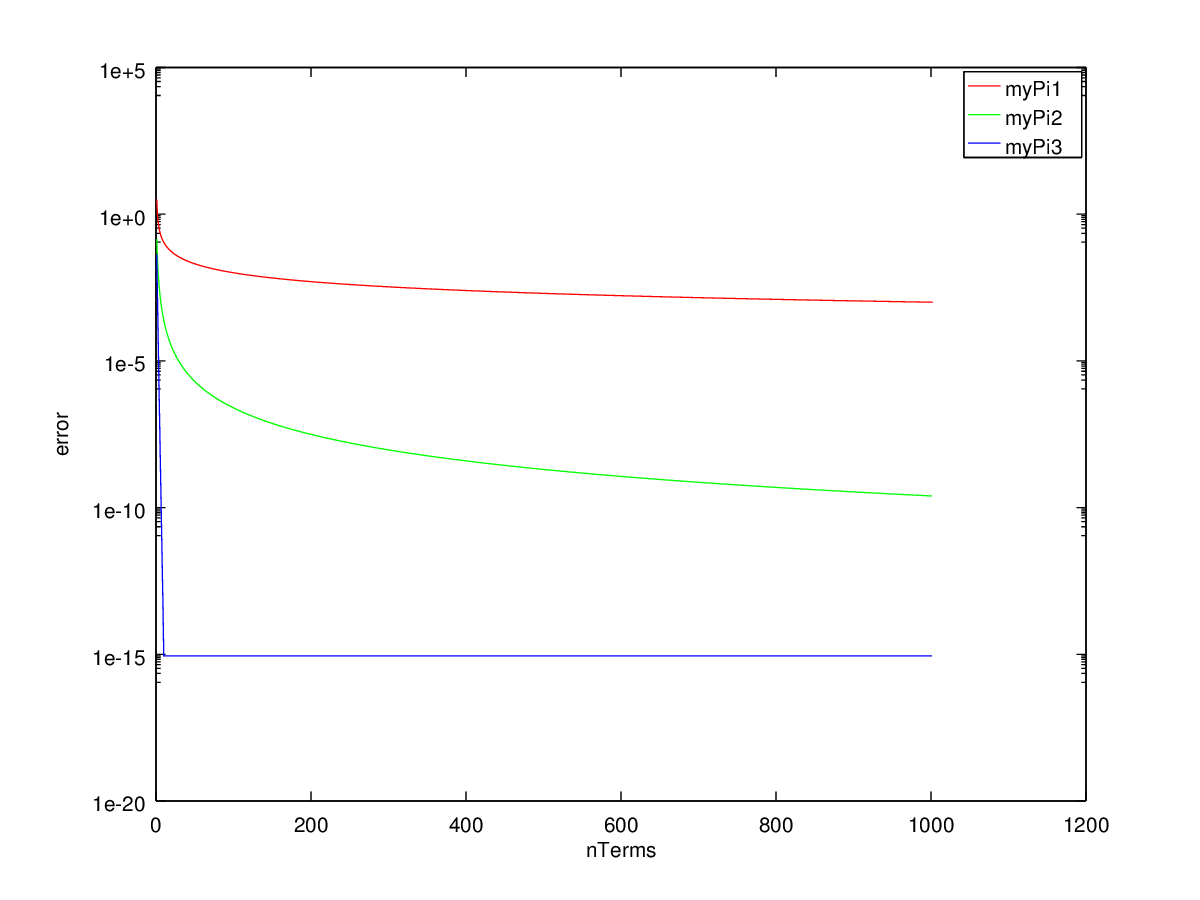
\includegraphics[scale=0.7]{pichart}
\end{center}

\subsection*{Assignment 1c. Decimal to Ternary conversion}
Modify the example function \verb=decInt2BinInt(x, nbits)= given in the lecture to  
a function that converts decimal integer to ternary integer (base-3): \verb=decInt2TerInt(x, nbits)=.

\paragraph{Solution}
\begin{verbatim}
function m = decInt2TerInt(decInt, nbits)
  m = zeros(1,nbits);
  for i = 1:nbits
    quotient = floor(decInt/3);
    m(nbits+1-i) = decInt-3*quotient;
	  decInt = quotient;
  endfor
  if decInt !=0
    fprintf("overflow.\n");
  endif
endfunction
\end{verbatim}
\end{document}
